\documentclass[
  11pt,
  letterpaper,
   addpoints,
   answers
  ]{exam}

\usepackage{../exercise-preamble}

\begin{document}

\noindent
\begin{minipage}{0.47\textwidth}

\includegraphics[width=\textwidth]{../fcfm_die}
\end{minipage}
\begin{minipage}{0.53\textwidth}
\begin{center} 
\large\textbf{Conversion de la energia y sistemas Electricos} (EL3103) \\
\large\textbf{Tarea 1} \\
\normalsize Prof.~Constanza Ahumada - Rodrigo Moreno V.\\
\normalsize Prof.~Aux.~Javiera Pacheco - Erik Saez.
\normalsize Ayudantes.~Manuel Aceituno - Pamela Acuña - Alvaro Flores 
\end{center}
\end{minipage}

\vspace{0.5cm}
\noindent
\vspace{.85cm}
\hrule
\textbf{Indicacciones: La tarea se puede realizar en grupos de - . Debe ser entregada el dia - , no se aceptan atrasos, el formato debera ser tipo informe.}
\hrule
\noindent
\vspace{.85cm}
\begin{questions}
    %%%%%%%%%%%%%%%%%%%%%%%%%%%
    \question Un amigo suyo se enteró que podía tener un cartel de permeabilidad magnética infinita y masa bien distribuida de 0.1 [kg] levitando gracias al poder del electromagnetismo, por ello le pidió que le calcule la corriente necesaria para poder lograr su cometido. El circuito magnético que posee está compuesto por dos núcleos magnéticos semicirculares de iguales dimensiones, con la disposición que se ve en la figura, tienen radio interno 6 [cm], radio externo 8 [cm] y profundidad de 2 [cm], lamentablemente estos tienen distinta permeabilidad relativa siendo esta $u_{r}=2$ para el núcleo asociado a la primera bobina y $u_{r}=3$ para la segunda.
    \begin{figure}[h!]
        \centering
        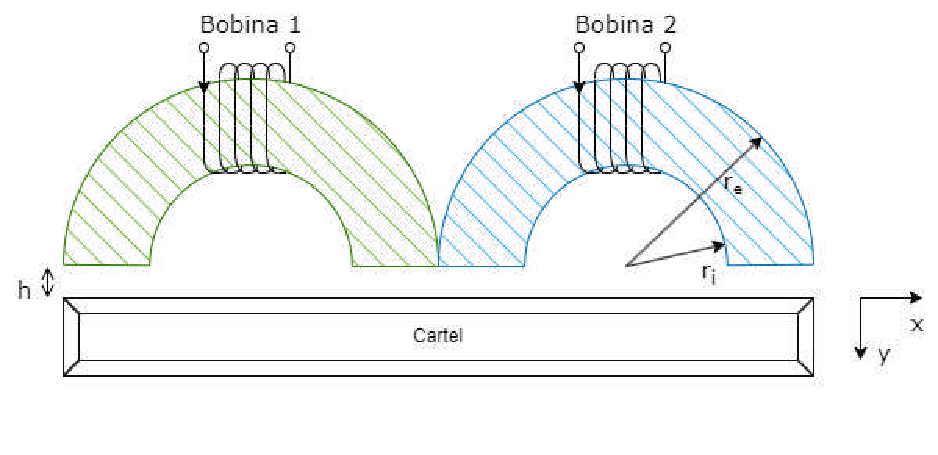
\includegraphics[width=0.5\textwidth]{Tarea_1_1}
    \end{figure}
    \begin{itemize}
        \item \textbf{(1.5 Puntos)} Calcule el circuito equivalente del sistema, calcule las reluctancias de los elementos presentes y la inductancia propia de cada bobina.
        \item \textbf{(2 Puntos)} Su amigo es muy perfeccionista así que el cartel no puede quedar desnivelado, encuentre la relación que deben cumplir las fuerzas magnetomotrices para ello.
        \item \textbf{(2 Puntos)} Su amigo le menciona que las bobinas de 200 vueltas estaban a 2x1 por ello las compró, le gustaría que el cartel levite a 3mm de los núcleos que están fijos, con esta información, encuentre las corrientes que deben circular por cada bobina (Indicación: La fuerza ejercida por un sistema puede calcularse como la derivada de la energía del sistema respecto a la posición (h))
        \item \textbf{(0.5 Puntos)} Respecto a las corrientes que encontró, entregue su opinión a su amigo.
    \end{itemize}
    %%%%%%%%%%%%%%%%%%%%%%%%%%%

    %%%%%%%%%%%%%%%%%%%%%%%%%%%
    \question Para mantener el voltaje en bornes de un generador síncrono, Con el fin de poder variar el voltaje $v_{o}$ del
    campo del generador síncrono se utiliza un conversor AC/DC como se muestra en la Figura 3.
    \begin{figure}[h!]
        \centering
        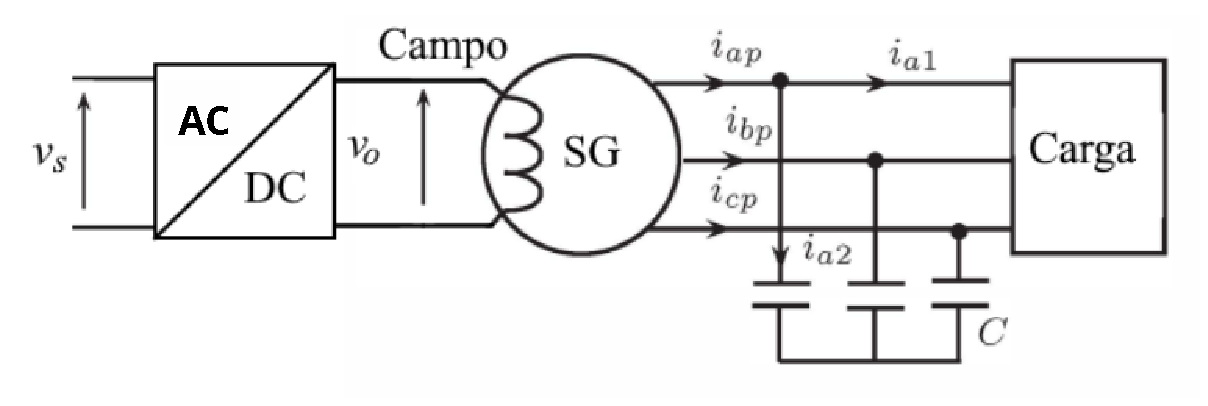
\includegraphics[width=0.5\textwidth]{Tarea_1_2}
    \end{figure}
    \begin{itemize}
        \item \textbf{(0.5 Puntos)} Dado el esquema visto en la figura anterior, fabrique el conversor AC/DC , para obtener una $V_{o}= 120[V]$ mediante un rectificador de onda completa monofásico. Considere que la frecuencia de la red es de $60[Hz]$ y que su condensador es de $C=1[F]$, debe obtener los graficos asociados a la señal de salida y la señal de entrada.
        \item \textbf{(0.5 Puntos)} Realice el mismo procedimiento pero para un rectificador de onda completa trifásico.
        \item \textbf{(1 Puntos)} Debido a nuevas tecnologias, se desea implimentar un rectificador controlado monofásico. ¿Cuál es el valor de $\alpha$ para obtener una señal de salida de $V_{o}= 120[V]$?. Se debe justificar la razon de la eleccion del \textit{Duty cicle} y como este afecta su respuesta.
        \item \textbf{(1 Puntos)}Realice el mismo procedimiento pero para un rectificador controlado trifásico.
        \item \textbf{(3 Puntos)} Investigacion
    \end{itemize}
\end{questions}
Para la realizacion de la tarea se puede utilizar el software de simulacion que estime conveniente (\textit{Recomiendo personalmente PLECS}). Todo los graficos deben estar bien rotulados , ademas mostrar los esquemas realizados en la simulacion como los parametros utilziados.
\end{document}